\chapter{Validation}
\label{chp:validation}
% Probably the biggest chapter:
% - explain the metrics
% - explain the scenarios
% - display the good and bad results (highlight both)
% - display the high level results

% Why is validation needed?
Chapter in which the validation will reside.

\section{Metrics used}
To validate this project correctly, the metrics that are worked with must be established. Once the metrics are familiar, some metrics can be changed from one scenario to another, while some of the metrics remain the same. In this way, it can be determined which metric has an impact on the accuracy of the sensor. 

\subsection{Recorded metrics}
The recorded metrics are the measurements that are being taken to measure the vital signs for a person. These measurements are coming from the sensor, but also from other devices to validate the measurements from the sensor. The sensor itself measures the heartrate and respiration rate from one or multiple persons. But not only this information gets send back to the computer. To make the visualization on the computer a bit better, different waveforms are also send to the computer. There is one unfiltered waveform, a heartrate waveform and a respiration rate waveform. The unfiltered waveform is the phase of the radar data for the bin in which the measured person is residing. The heartrate and respiration rate waveforms are the waveforms from which the heartrate and respiration rate can be determined. These waveforms are being generated after the filtering of the phase signal, see also Section~\ref{sec:vit_signs_est}. 

\subsubsection{Heartrate validation}
The sensor does output a heartrate, but there also needs to be a method to validate this heartrate measurement. This is done by also connecting the measured person to an SpO2 sensor. The exact workings of this sensor are also explained in Section~\ref{sec:spo2_sensors}. This sensor outputs two metrics: heartrate and blood oxygen levels. The only metric which is used for this project is the heartrate. The SpO2 sensor used in this project is the \emph{Nonin 9600}, see also Figure~\ref{fig:nonin_9600}. This device has been chosen for various reasons. It is a medical grade device, which means that it is build following a high standard, and the measurements outputted by the sensor must have very low tolerances. This device also has a serial port. Each second, the device outputs the heartrate and respiration rate to the serial bus. This data stream can very easily be captured using a RS232 to USB converter, and saved to a file for later use. The only problem is that there are only two devices available. This is enough for a thorough evaluation of the vital signs estimation and also for measurements of two persons at the same time, but not for four persons. During the test with measuring four persons at the same time, two other SpO2 sensors were used, the \emph{iHealth Air Pulse Oximeter}, see Figure~\ref{fig:ihealth}. These sensors don't have a connection available to send the data to a computer, so the sensors are read every minute, and the reading from the sensor is recorded. 

\begin{figure}[t]
    \centering
    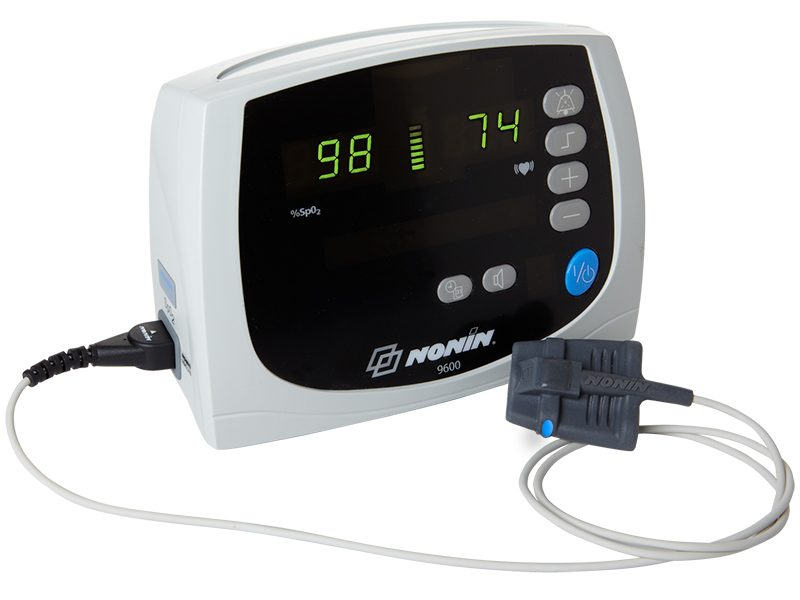
\includegraphics[width=.6\textwidth]{figures/validation/nonin_9600.jpg}
    \caption{The Nonin 9600 SpO2 sensor used as validation in this project.}
    \label{fig:nonin_9600}
\end{figure}

\begin{figure}[t]
    \centering
    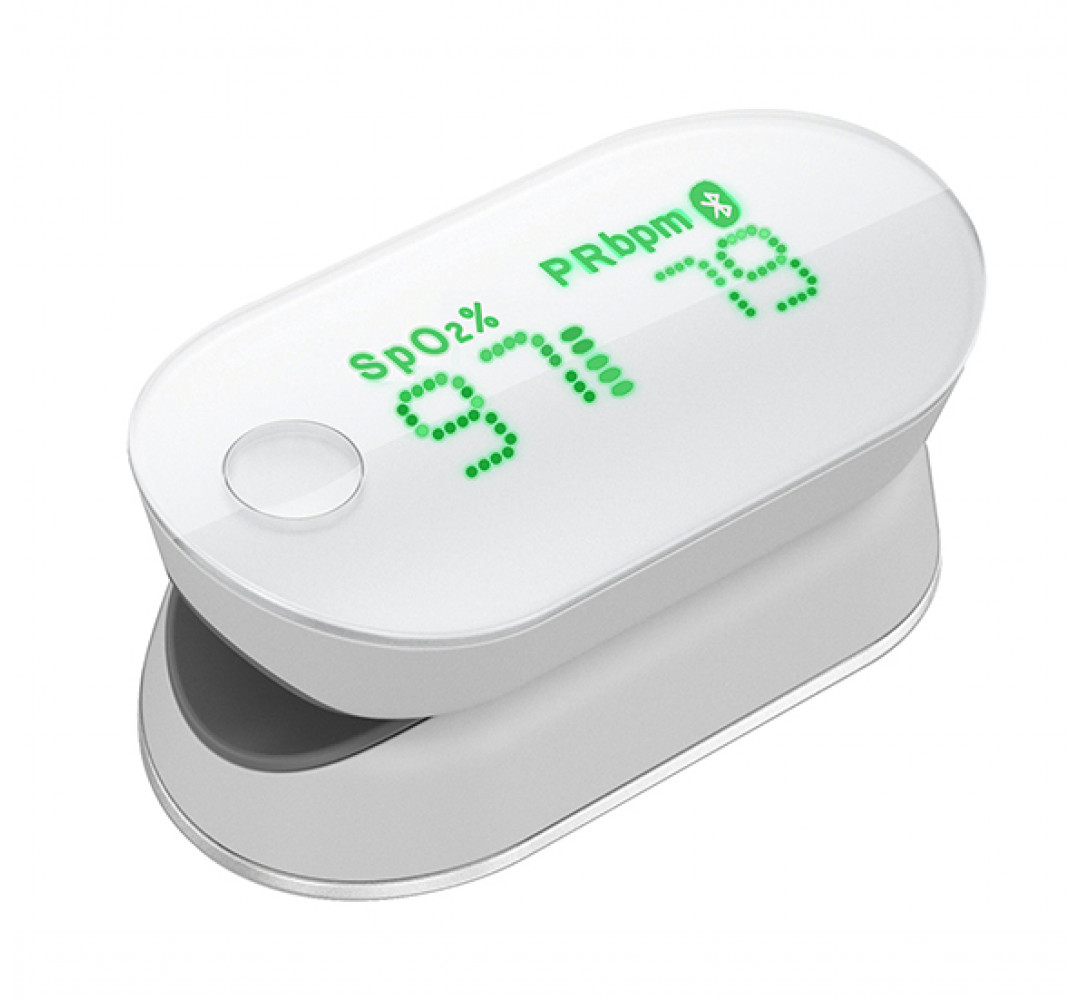
\includegraphics[width=.4\textwidth]{figures/validation/ihealth.jpg}
    \caption{The iHealth Air Pulse Oximeter used as validation in this project.}
    \label{fig:ihealth}
\end{figure}

\subsubsection{Respiratory validation}
While there are certainly devices which could measure respiration rate of a person, these devices were not present in the Erasmus MC hospital, where the tests were performed. To still validate the respiration rate of a person, the following validation technique was developed. Since the person being measured is only sitting in front of the sensor and not doing any activities, the person is asked to count its own breathing. Every breath in and out counts as one breath, and each minute, this value is recorded and the counting starts again. This value counts as the validation for the respiration rate outputted by the IWR6843. This method has its downsides, people could forget to count, they could make a counting mistake, or they could start breathing non-naturally, since they are focusing on their breath. This is still the best way to measure the respiration rate during the project, but these downsides must be kept in mind when analyzing the validation results.

\subsection{External metrics}
Metrics outside of the sensor could also have an effect on the quality of the measurements. These metrics contain among others the position in front of the sensor, the amount of people in front of the sensor and movement in the room.

\subsubsection{Position with respect to the sensor}
The IWR6843 is set up to measure persons within 0.3 to 0.9 meter range of the sensor, in the whole azimuth range, see also Figure~\ref{fig:range_metric}. The position of the person in the field of view of the sensor could play a role in the accuracy of the measurements.

\begin{figure}[t]
    \centering
    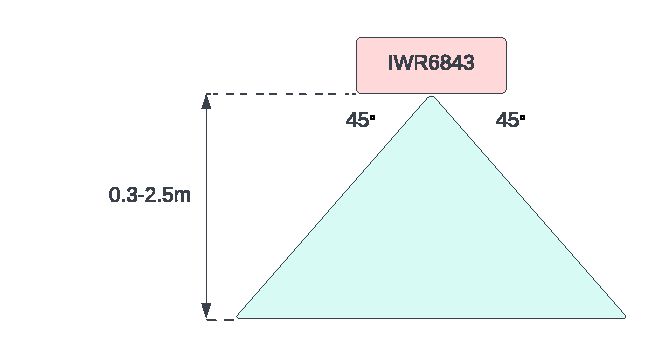
\includegraphics[width=.6\textwidth]{figures/validation/range_metric.pdf}
    \caption{Range and azimuth constraints of the sensor.}
    \label{fig:range_metric}
\end{figure}

\subsubsection{Amount of persons in front of the sensor}
The amount of persons that need to be measured is also a metric. It is possible that measurements of multiple persons close to each other will interfere.

\subsubsection{Background noise}
The sensor is very sensitive to noise. For the best result, the person needs to sit very still, and there needs to be as less noise as possible in the field of view of the sensor.

\subsubsection{Height of the sensor}
The height of the sensor with respect to the chest region of the measured persons is very important. The sensor needs to be at the same height as the middle of the chest of the measured persons. Otherwise, the vibrations of the chest can't be picked up by the sensor and the measurements become unreliable.

\subsection{Person metrics}
\label{sec:person_metrics}
The persons for which the vital signs are measured, all have different attributes. The most important ones are:

\begin{itemize}
    \item \textbf{gender:} there exist physical differences between men and women, also in the chest region where this project is focusing on. This metric could determine if men and woman are easier or more difficult to measure.
    \item \textbf{age:} the age of a person could contribute to multiple factors. A child is small, has a small chest region and could have a faster beating heart. Older persons are more likely to have extra body fat to dampen the vibrations produced by the heart and lungs.
    \item \textbf{weight/BMI:} body mass could have a big impact on the measurements. Positively, persons with a bigger weight are more likely to have a bigger chest region, so are easier to measure. Negatively, persons with more body mass are more likely to have extra fat on top of the chest, which could dampen the vibrations caused by the heart and lungs.
\end{itemize}

\section{Testing setup}
\label{sec:test_setup}
The testing environment is kept as consistent as possible. All of the equipment is placed on a desk, and in front of the desk one or more chairs are placed. The IWR6843 is set on the desk, with the antennae pointing to the chairs. Next to the IWR6843 the two Nonin 9600 SpO2 sensors are placed, since the sensor leads are not that long. The IWR6843 and the two SpO2 sensors are connected to the computer via serial buses. The computer is operated by the operator. See also Figure~\ref{fig:test_setup} and Figure~\ref{fig:test_setup_pic}.

All tests have a duration of 5 minutes, or 300 seconds. The amount of 300 seconds has been chosen for multiple reasons. It gives the sensor time to stabilize. Because multiple buffers are used inside of the sensor, it takes some time before the buffers are filled with valid measurement data. Because the test subjects have walked to the testing location, it also gives the heartrate of the test subjects some time to settle in the heartrate during rest, which is the most stable.

\begin{figure}[t]
\begin{subfigure}{.45\textwidth}
  \centering
  % include first image
  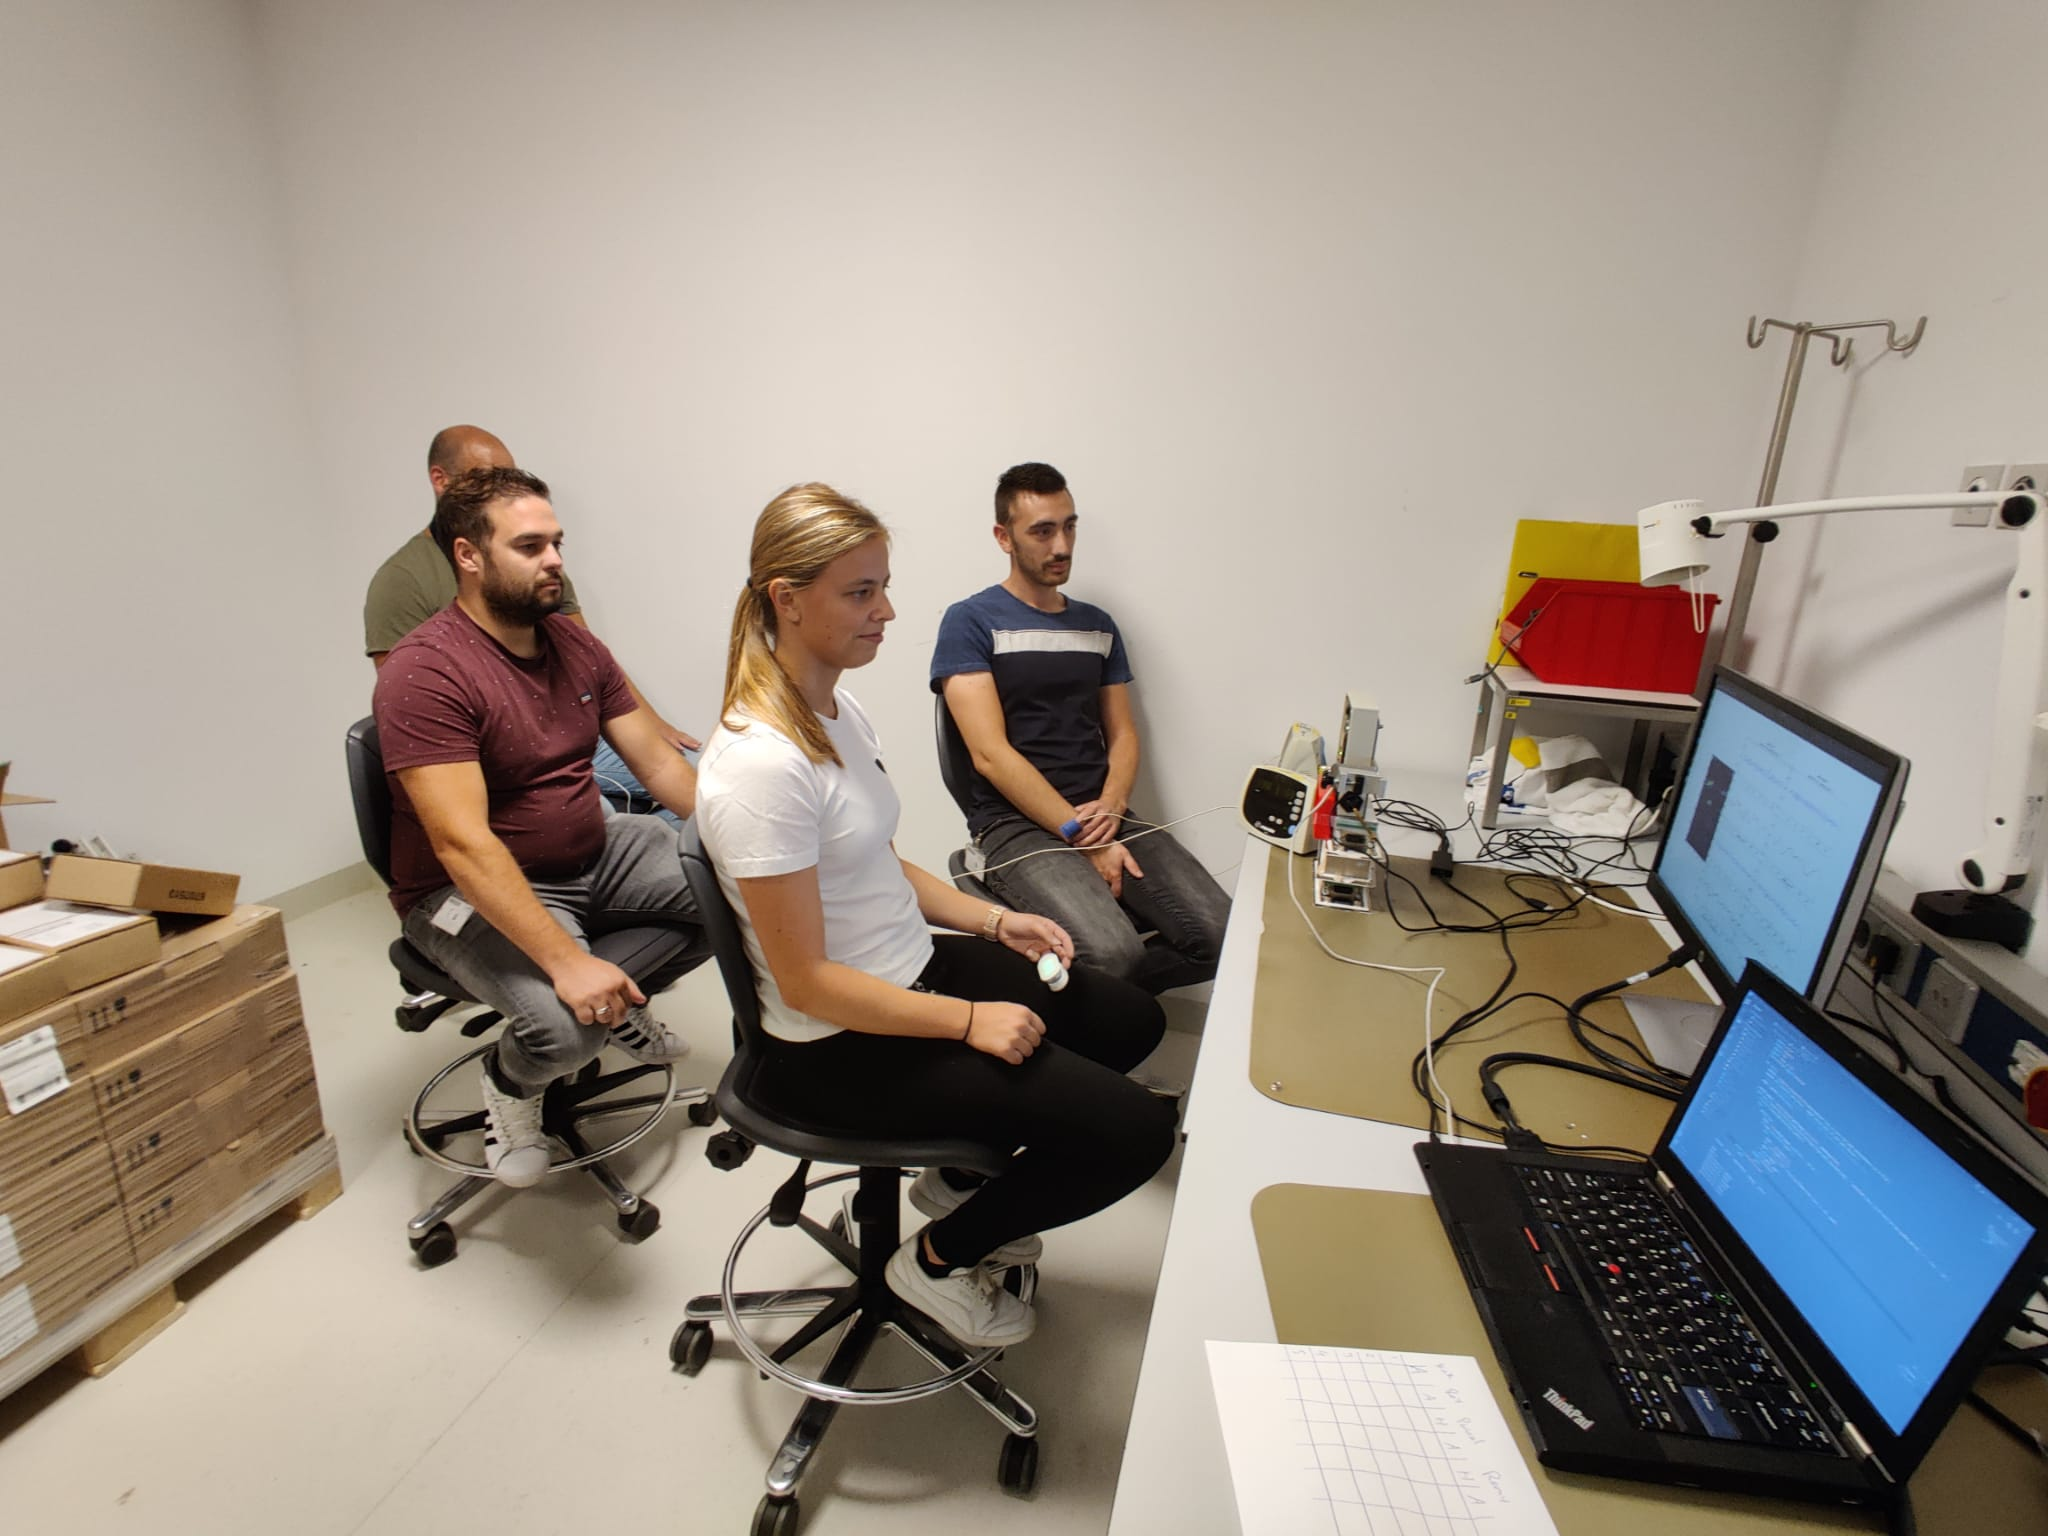
\includegraphics[width=\linewidth]{figures/validation/layout_4pers.jpeg}  
  \caption{Picture taken during the 4 persons vital sign estimation test.}
  \label{fig:test_setup_4_pic}
\end{subfigure}
\begin{subfigure}{.45\textwidth}
  \centering
  % include second image
  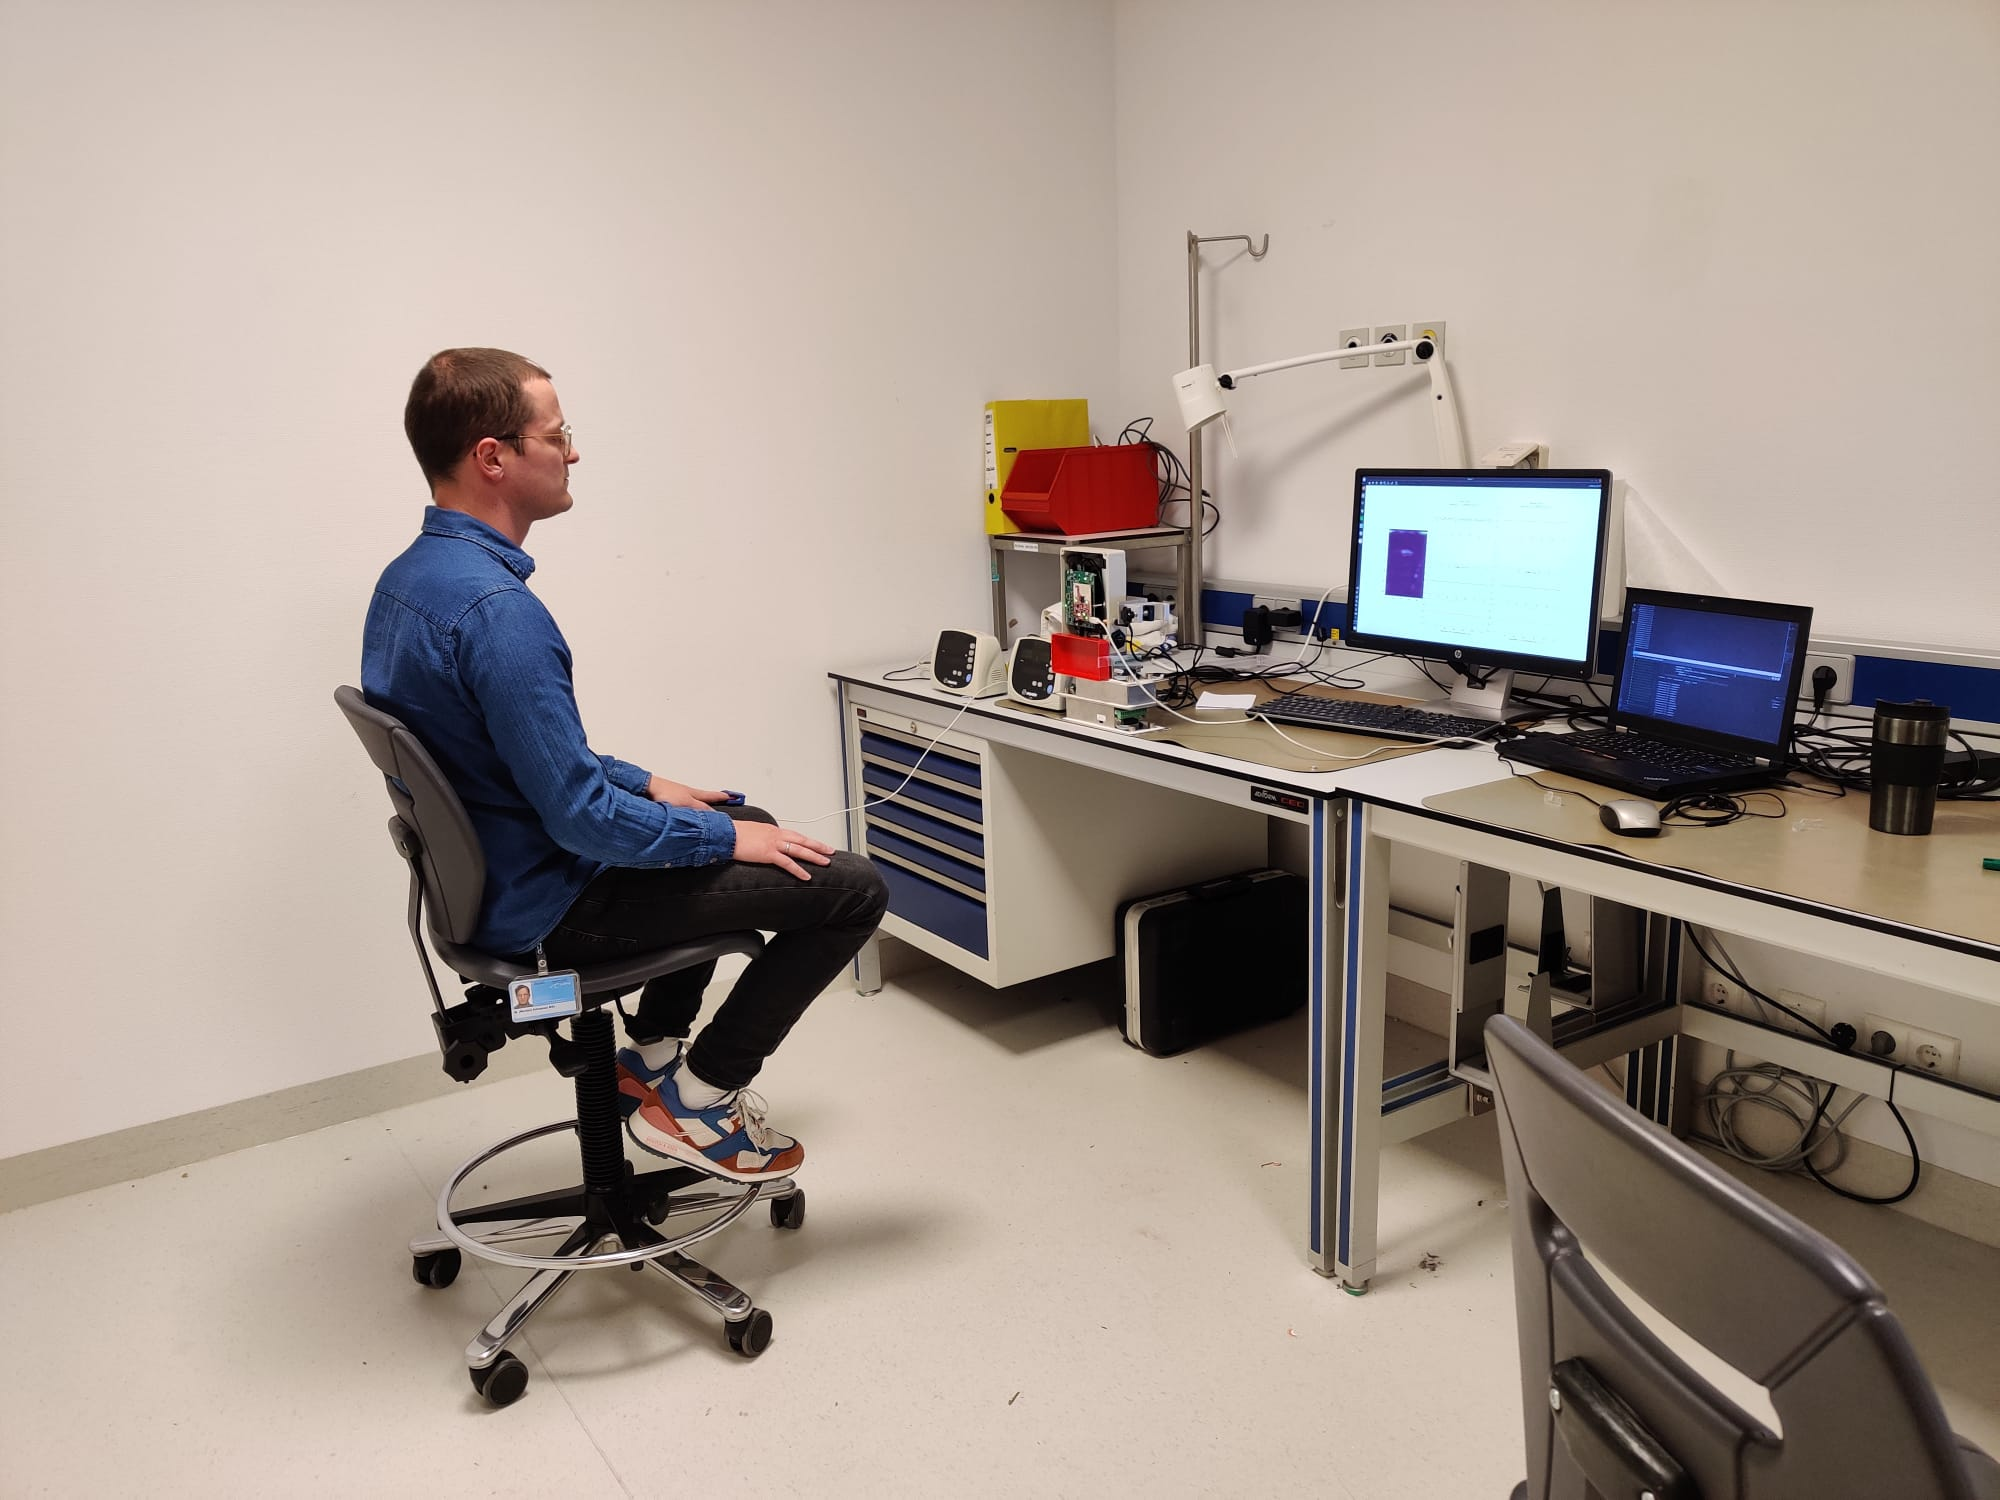
\includegraphics[width=\linewidth]{figures/validation/layout_michiel.jpeg}  
  \caption{Picture taken during the 1 person vital sign estimation test.}
  \label{fig:test_setup_1_pic}
\end{subfigure}
\caption{Two different tests being executed.}
\label{fig:test_setup_pic}
\end{figure}

\begin{figure}[t]
\begin{subfigure}{\textwidth}
  \centering
  % include first image
  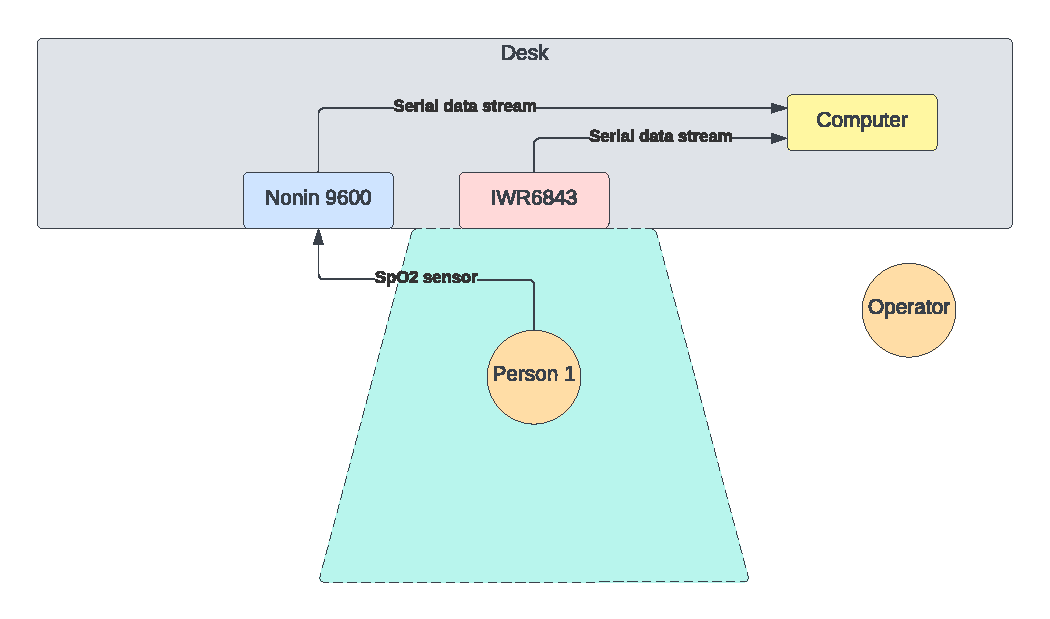
\includegraphics[width=.6\linewidth]{figures/validation/test_setup_1.pdf}  
  \caption{Test setup for vital sign estimation of 1 person.}
  \label{fig:test_setup_1}
\end{subfigure}
\begin{subfigure}{\textwidth}
  \centering
  % include second image
  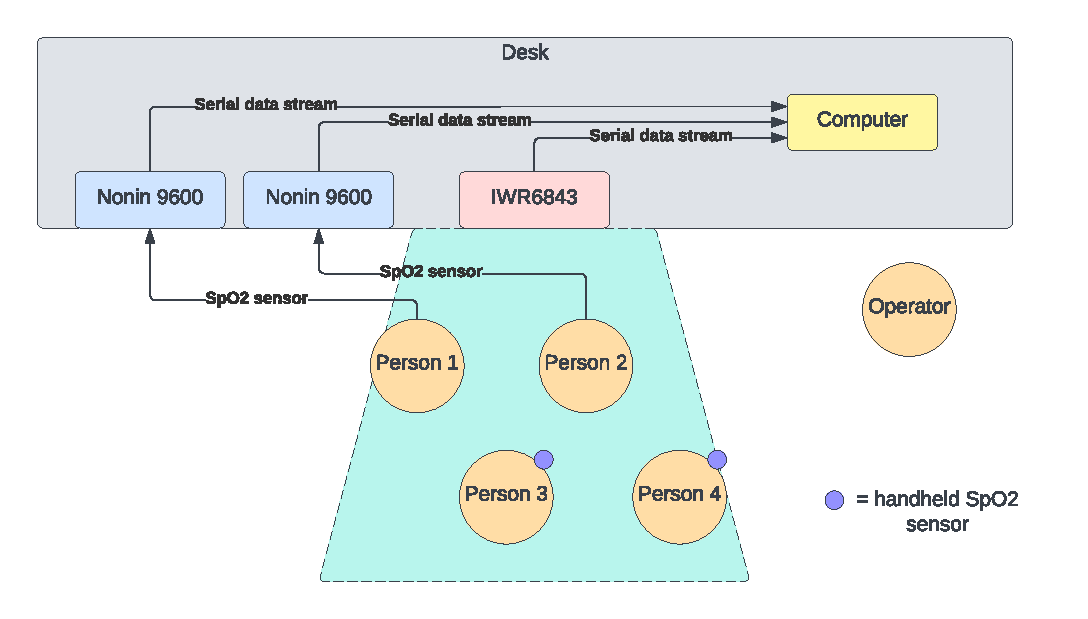
\includegraphics[width=.6\linewidth]{figures/validation/test_setup_4.pdf}  
  \caption{Test setup for the vital sign estimation of 4 persons.}
  \label{fig:test_setup_4}
\end{subfigure}
\caption{Two test setups being used to validate the project.}
\label{fig:test_setup}
\end{figure}

\section{Test subjects}
To properly validate the sensor, it has to be tested on persons. These test subjects were selected to reflect the validation plan. Most of the test subjects were colleges, family or friends. The test subjects are recorded for 5 minutes in a row, and along with the measurement data, additional metadata of the test subjects was recorded, as described in Section~\ref{sec:person_metrics}. This data includes age, gender, weight, length and additional comments. Using the weight and length, the BMI can be calculated. This data can be found in Table~\ref{tab:persons-info}.

Because the data which is being recorded is highly sensitive medical data, the names of the persons are anonymized. All of the persons also have signed an informed consent. The informed consent forms can be found in Appendix \todo{Add the informed consent forms to the appendix.}. 

\begin{table}[ht]
\centering
\begin{tabular}{|l|l|l|l|l|l|l|}
\hline
Name & Age & Gender & \begin{tabular}[c]{@{}l@{}}Weight \\ (kg)\end{tabular} & \begin{tabular}[c]{@{}l@{}}Length \\ (m)\end{tabular} & BMI & Comments \\ \hline
P1 & 23 & male & 72 & 1.75 & 23 &  \\
P2 & 61 & female & 78 & 1.60 & 30 &  \\
P3 & 32 & male & 75 & 1.85 & 21 &  \\
P4 & 25 & male & 80 & 1.80 & 24 & \begin{tabular}[c]{@{}l@{}}Wore big layers \\ of clothing\end{tabular} \\
P5 & 26 & male & 100 & 1.80 & 30 & \begin{tabular}[c]{@{}l@{}}P5 was not detected \\ very well by the sensor\end{tabular} \\
P6 & 27 & male & 70 & 1.75 & 22 & Has a high metabolism \\
P7 & 23 & male & 90 & 1.82 & 27 & \begin{tabular}[c]{@{}l@{}}Was a bit restless during \\ testing, has a big heart\end{tabular} \\
P8 & 43 & male & 80 & 1.82 & 24 &  \\
P9 & 49 & male & 85 & 1.85 & 24 & Lung problems \\
P10 & 35 & male & 86 & 1.77 & 27 &  \\
P11 & 49 & male & 92 & 1.80 & 28 &  \\
P12 & 23 & female & 62 & 1.75 & 20 &  \\
P13 & 76 & male & 91 & 1.75 & 29 &  \\
P14 & 75 & female & 82 & 1.65 & 30 &  \\ \hline
\end{tabular}
\caption{All of the recorded metadata from the test subjects.}
\label{tab:persons-info}
\end{table}

\section{Results}
\subsection{One person validation}
\label{sec:one_pers_validation}
The validation of the vital signs of one person in front of the sensor is an important part of the validation process. Because the vital sign estimation of one person is the same process as the vital sign estimation of multiple persons, the validation of one person already says a lot about the validation of multiple persons. To validate the general accuracy of the project, 11 persons have been tested, all individually. The test setup can be found in Section~\ref{sec:test_setup}. 

For each recorded heartrate and respiration rate from the IWR6843, it is compared against the true heartrate and respiration rate. For each test subject, the average deviation percentage is calculated. The deviation percentage is how much the measurement from the IWR6843 differs from the control measurement. The percentage is calculated using this formula:

\begin{equation}
    deviation = abs(M_{IWR6843} - M_{control}) / M_{control}
    \label{eq:deviation_calculation}
\end{equation}

These percentages can be found in Table~\ref{tab:one-person-results}\todo{Incorporate averages from the whole measurement?}. The measurements for each test subject can also be plotted, but that takes up too much space. So, only the most accurate measurement and the least accurate measurement are drawn in this thesis. For the most accurate result, see Figure~\ref{fig:roy_meas}. For the least accurate result, see Figure~\ref{fig:tim_meas}\todo{Replace with P13?}.

\begin{table}[ht]
\centering
\begin{tabular}{|r|c|c|l|}
\hline
Person & \begin{tabular}[c]{@{}c@{}}Heartrate \\ accuracy\end{tabular} & \begin{tabular}[c]{@{}c@{}}Respiratory \\ rate accuracy\end{tabular} & \textbf{Average} \\ \hline
P1 & 8.22\% & 6.56\% & \textbf{7.39\%} \\
P2 & 1.71\% & 9.53\% & \textbf{5.62\%} \\
P3 & 4.70\% & 2.01\% & \textbf{3.35\%} \\
P4 & 29.75\% & 11.11\% & \textbf{20.43\%} \\
P5 & 16.74\% & 8.51\% & \textbf{12.63\%} \\
P6 & 5.49\% & 15.74\% & \textbf{10.62\%} \\
P7 & 20.61\% & 23.93\% & \textbf{22.27\%} \\
P8 & 16.85\% & 13.49\% & \textbf{15.17\%} \\
P9 & 24.80\% & 7.89\% & \textbf{16.35\%} \\
P13 & 35.39\% & 13.12\% & \textbf{24.26\%} \\
P14 & 18.81\% & 16.64\% & \textbf{17.72\%} \\ \hline
\textbf{Average} & \textbf{17.44\%} & \textbf{13.72\%} & \textbf{15.58\%} \\ \hline
\end{tabular}
\caption{One person vital signs estimation validation results. The percentage denotes the absolute difference between the IWR6843 heart- and respiration rate, and the control rates.}
\label{tab:one-person-results}
\end{table}

\begin{table}[ht]
\centering
\begin{tabular}{|r|c|c|l|c|c|l|}
\hline
Person & \begin{tabular}[c]{@{}c@{}}Heartrate \\ SpO2 \\ sensor\end{tabular} & \begin{tabular}[c]{@{}c@{}}Heartrate\\ IWR6843\end{tabular} & \textbf{\begin{tabular}[c]{@{}l@{}}Heartrate\\ deviation\end{tabular}} & \textbf{\begin{tabular}[c]{@{}c@{}}Respi-\\ ratory\\ rate\end{tabular}} & \textbf{\begin{tabular}[c]{@{}c@{}}Respi-\\ ratory\\ rate \\ IWR6843\end{tabular}} & \textbf{\begin{tabular}[c]{@{}l@{}}Respi-\\ ratory\\ rate \\ deviation\end{tabular}} \\ \hline
P1 & 71 & 65 & \textbf{8.03\%} & 10 & 9 & \textbf{6.70\%} \\
P2 & 81 & 81 & \textbf{0.54\%} & 14 & 13 & \textbf{6.90\%} \\
P3 & 56 & 56 & \textbf{1.26\%} & 11 & 11 & \textbf{0.54\%} \\
P4 & 83 & 62 & \textbf{25.83\%} & 8 & 8 & \textbf{2.82\%} \\
P5 & 66 & 59 & \textbf{10.77\%} & 15 & 13 & \textbf{8.29\%} \\
P6 & 75 & 76 & \textbf{1.36\%} & 6 & 7 & \textbf{14.22\%} \\
P7 & 66 & 63 & \textbf{3.59\%} & 6 & 7 & \textbf{19.19\%} \\
P8 & 60 & 57 & \textbf{3.80\%} & 9 & 9 & \textbf{7.61\%} \\
P9 & 80 & 60 & \textbf{24.48\%} & 15 & 15 & \textbf{4.61\%} \\
P13 & 94 & 61 & \textbf{35.26\%} & 11 & 10 & \textbf{7.82\%} \\
P14 & 69 & 66 & \textbf{4.54\%} & 10 & 10 & \textbf{5.00\%} \\
\textbf{Average} & \textbf{} & \textbf{} & \textbf{10.86\%} &  &  & \textbf{7.61\%} \\ \hline
\end{tabular}
\caption{One person vital signs estimation validation results. The average heartrates and respiratory rates of all sensors from the whole reading, with the absolute deviation between the control measurements and the IWR6843 measurements.}
\label{tab:one-person-results_2}
\end{table}

\begin{figure}[t]
\begin{subfigure}{\textwidth}
  \centering
  % include first image
  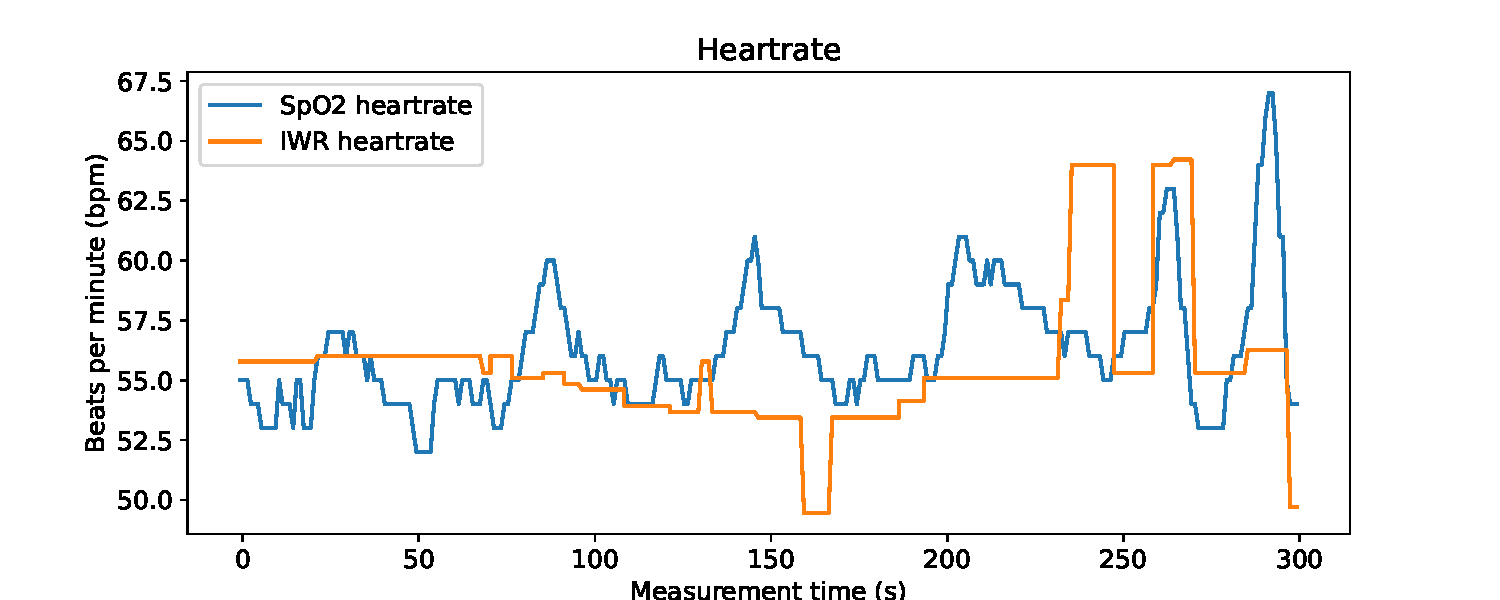
\includegraphics[width=\linewidth]{figures/validation/roy_heart.pdf}  
  \caption{The IWR6843 estimated heartrate and the SpO2 sensor heartrate from \emph{P3} plotted out.}
  \label{fig:roy_heart}
\end{subfigure}
\begin{subfigure}{\textwidth}
  \centering
  % include second image
  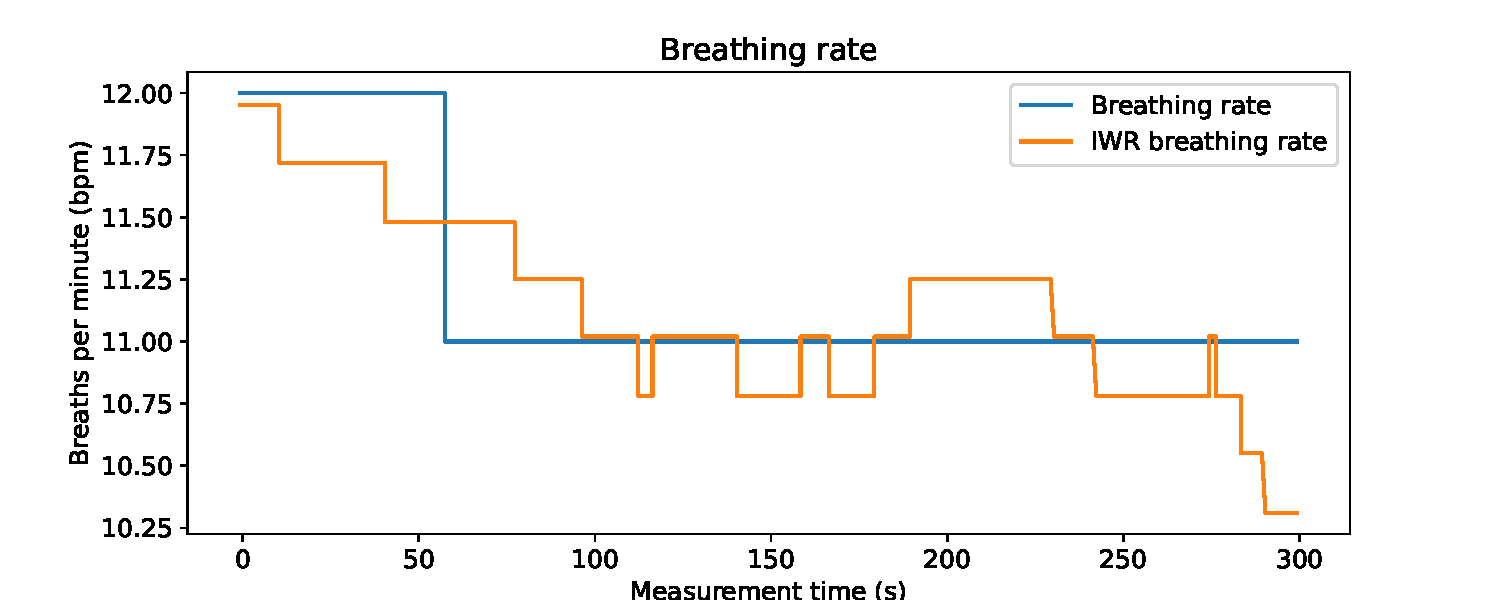
\includegraphics[width=\linewidth]{figures/validation/roy_breath.pdf}  
  \caption{The IWR6843 estimated respiratory rate and the counted respiratory rate from \emph{P3} plotted out.}
  \label{fig:roy_breath}
\end{subfigure}
\caption{Validation data from \emph{P3}. This is the most accurate result in the one person validation section.}
\label{fig:roy_meas}
\end{figure}

\begin{figure}[t]
\begin{subfigure}{\textwidth}
  \centering
  % include first image
  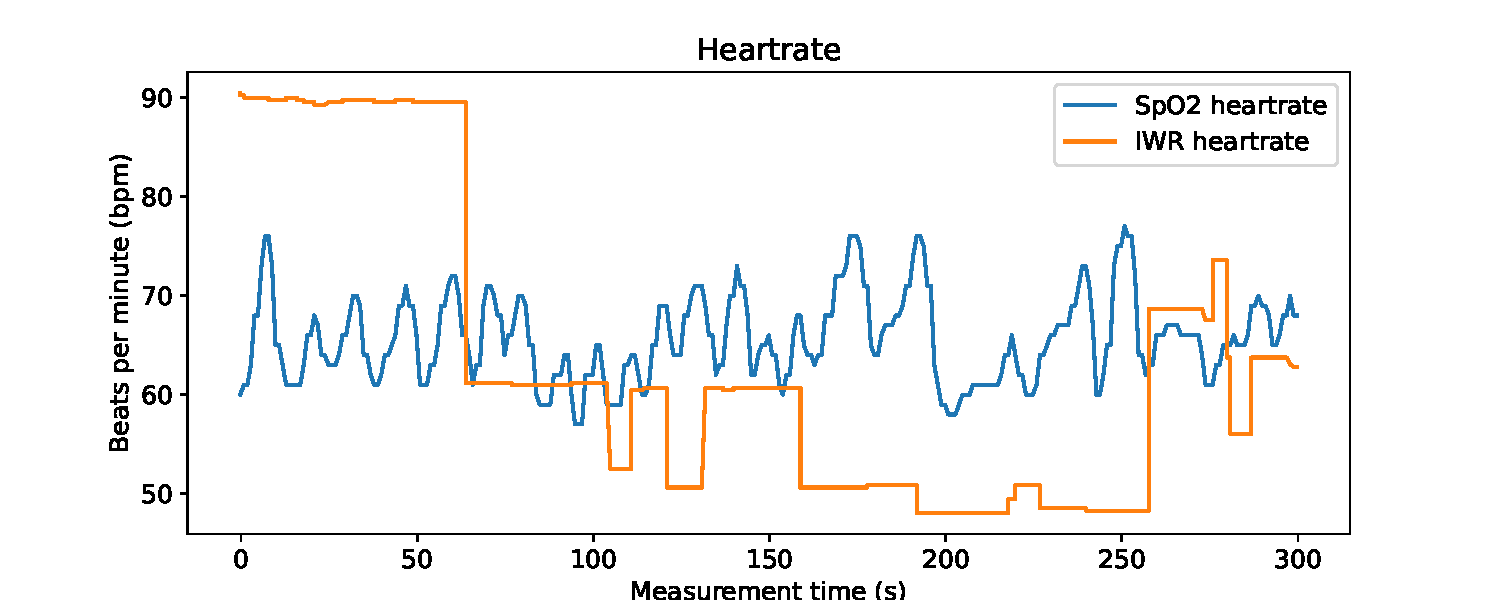
\includegraphics[width=\linewidth]{figures/validation/tim_heart.pdf}  
  \caption{The IWR6843 estimated heartrate and the SpO2 sensor heartrate from \emph{P7} plotted out.}
  \label{fig:tim_heart}
\end{subfigure}
\begin{subfigure}{\textwidth}
  \centering
  % include second image
  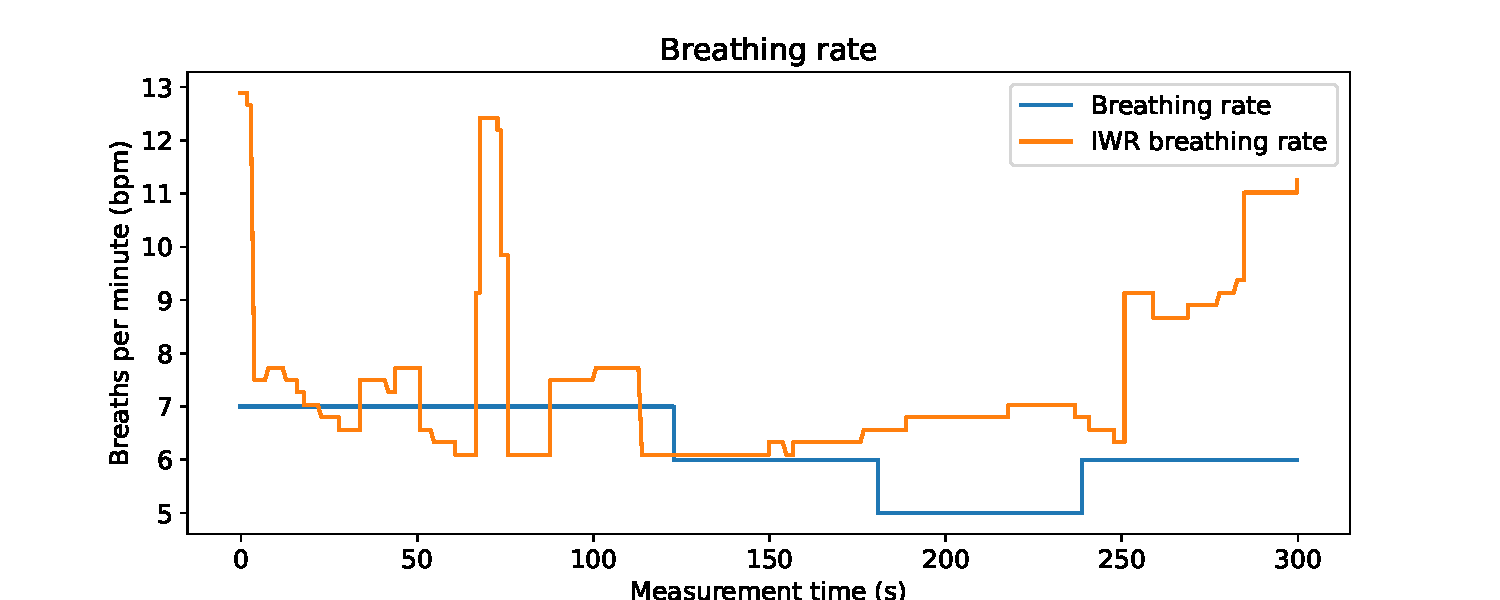
\includegraphics[width=\linewidth]{figures/validation/tim_breath.pdf}  
  \caption{The IWR6843 estimated respiratory rate and the counted respiratory rate from \emph{P7} plotted out.}
  \label{fig:tim_breath}
\end{subfigure}
\caption{Validation data from \emph{P7}. This is the least accurate result in the one person validation section.}
\label{fig:tim_meas}
\end{figure}

\subsection{Two person validation}
\todo{Tests need to be done}

\subsection{Four person validation}
% - How the validation was done
% - The results
% - difficulty with the people detection
% - less accurate results
For this project, estimating the vital signs of 4 persons at the same time is the maximum. There are two reasons for this number. Firstly, because of the amount of calculations this is all the chip can handle at the moment because of timing constraints. Secondly, because the measurements take place in the range of 0.5 to 1.0 meter from the sensor, it becomes too crowded in front of the sensor with more than 4 persons. 

To validate the accuracy of measuring four vital signs at the same time, four persons were put in front of the sensor, as can be observed in Figure~\ref{fig:test_setup_4} and Figure~\ref{fig:test_setup_4_pic}. The rest of the validation procedure stays the same, the test is run for 5 minutes with the persons sitting statically. All of the chests of the four persons are at the same height of the sensor antennae. 

The most uncertain part of this validation was if the person detection would work reliably. Not only one, but four persons must be detected and remain detected during the 5 minutes of testing time. Luckily, the person detection remained stable during the test, and apart from a few glitches the four persons remained detected during the test, see also Figure~\ref{fig:4_persons_detected}.

\begin{figure}[t]
    \centering
    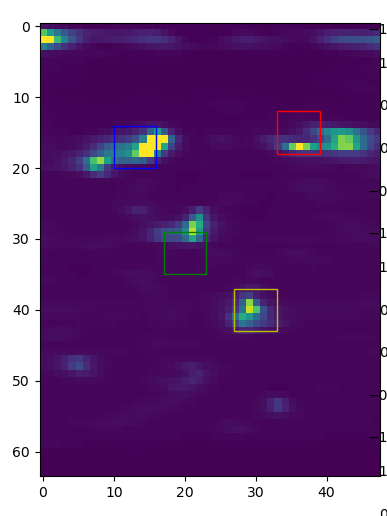
\includegraphics[width=.4\textwidth]{figures/validation/4personen_testen_crop.png}
    \caption{Four persons detected during the four person validation.}
    \label{fig:4_persons_detected}
\end{figure}

The graphs visualizing the measurement data for all four persons at the same time can be found in Figure~\ref{fig:4pers_heart_meas} and Figure~\ref{fig:4pers_breath_meas}. The most outstanding observation which can be done, is that the estimations from the IWR6843 are really jumping up and down. The measurements from the control group are much more stable. A positive observation is that the control measurement is most of the time approximately the average of the noisy measurements from the IWR6843. This is also confirmed with the numerical results in Table~\ref{tab:4pers_results} and Table~\ref{tab:4pers_results_2}. The numbers in this table are calculated in the same way as Section~\ref{sec:one_pers_validation}. In Table~\ref{tab:4pers_results}, each single result from the IWR6843 and the control group is compared to each other, which gives a large deviation because of the scattered results from the radar sensor. In Table~\ref{tab:4pers_results_2}, all measurements are averaged in one number. In this case, the deviation is much smaller.

\begin{table}[ht]
\centering
\begin{tabular}{|r|c|c|l|}
\hline
\textbf{Person} & \textbf{\begin{tabular}[c]{@{}c@{}}Heartrate\\ accuracy\end{tabular}} & \textbf{\begin{tabular}[c]{@{}c@{}}Respiratory\\ rate accuracy\end{tabular}} & \textbf{Average} \\ \hline
\textbf{P3} & 12.15\% & 21.53\% & \textbf{16.84\%} \\
\textbf{P10} & 21.19\% & 32.18\% & \textbf{26.69\%} \\
\textbf{P11} & 24.34\% & 25.18\% & \textbf{24.76\%} \\
\textbf{P12} & 18.06\% & 10.08\% & \textbf{14.07\%} \\ \hline
\textbf{Average} & \textbf{18.94\%} & \textbf{22.24\%} & \textbf{20.59\%} \\ \hline
\end{tabular}
\caption{Four person vital signs estimation validation results. The percentage denotes the absolute difference between the IWR6843 heart- and respiration rate, and the control rates.}
\label{tab:4pers_results}
\end{table}

\begin{table}[ht]
\centering
\begin{tabular}{|r|c|c|l|c|c|l|}
\hline
\textbf{Person} & \textbf{\begin{tabular}[c]{@{}c@{}}Heartrate\\ SpO2 \\ sensor\end{tabular}} & \textbf{\begin{tabular}[c]{@{}c@{}}Heartrate\\ IWR6843\end{tabular}} & \textbf{\begin{tabular}[c]{@{}l@{}}Heartrate\\ deviation\end{tabular}} & \textbf{\begin{tabular}[c]{@{}c@{}}Respi-\\ ratory\\ rate\end{tabular}} & \textbf{\begin{tabular}[c]{@{}c@{}}Respi-\\ ratory\\ rate\\ IWR6843\end{tabular}} & \textbf{\begin{tabular}[c]{@{}l@{}}Respi-\\ ratory\\ rate\\ deviation\end{tabular}} \\ \hline
\textbf{P3} & 61 & 64 & \textbf{5.64\%} & 7 & 9 & \textbf{28.24\%} \\
\textbf{P10} & 66 & 63 & \textbf{5.04\%} & 10 & 9 & \textbf{6.02\%} \\
\textbf{P11} & 69 & 58 & \textbf{16.09\%} & 8 & 9 & \textbf{2.38\%} \\
\textbf{P12} & 69 & 60 & \textbf{12.86\%} & 11 & 11 & \textbf{2.14\%} \\ \hline
\textbf{Average} &  &  & \textbf{9.91\%} &  &  & \textbf{9.70\%} \\ \hline
\end{tabular}
\caption{Four person vital signs estimation validation results. The average heartrates and respiratory rates of all sensors from the whole reading, with the absolute deviation between the control measurements and the IWR6843 measurements.}
\label{tab:4pers_results_2}
\end{table}

\begin{figure}[t]
\centering
\begin{subfigure}{.45\textwidth}
  \centering
  % include first image
  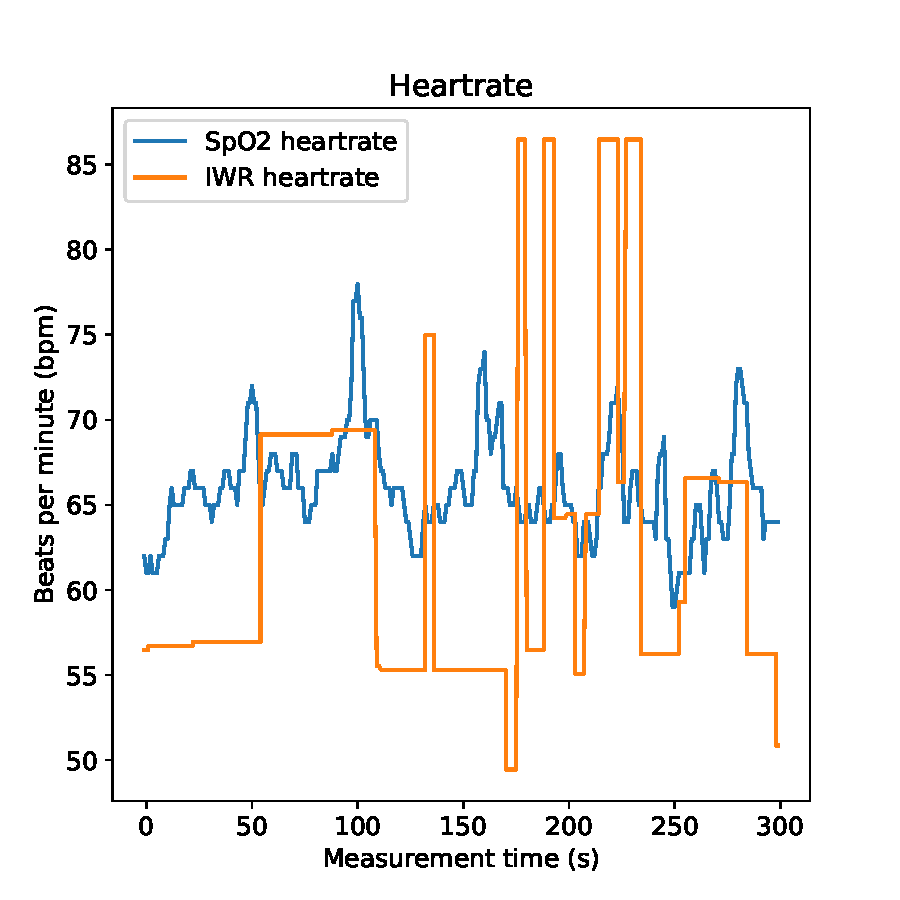
\includegraphics[width=\linewidth]{figures/validation/roy4_heart.pdf}  
  \caption{Heartrate of \emph{P3}}
  \label{fig:roy4_heart}
\end{subfigure}
\begin{subfigure}{.45\textwidth}
  \centering
  % include second image
  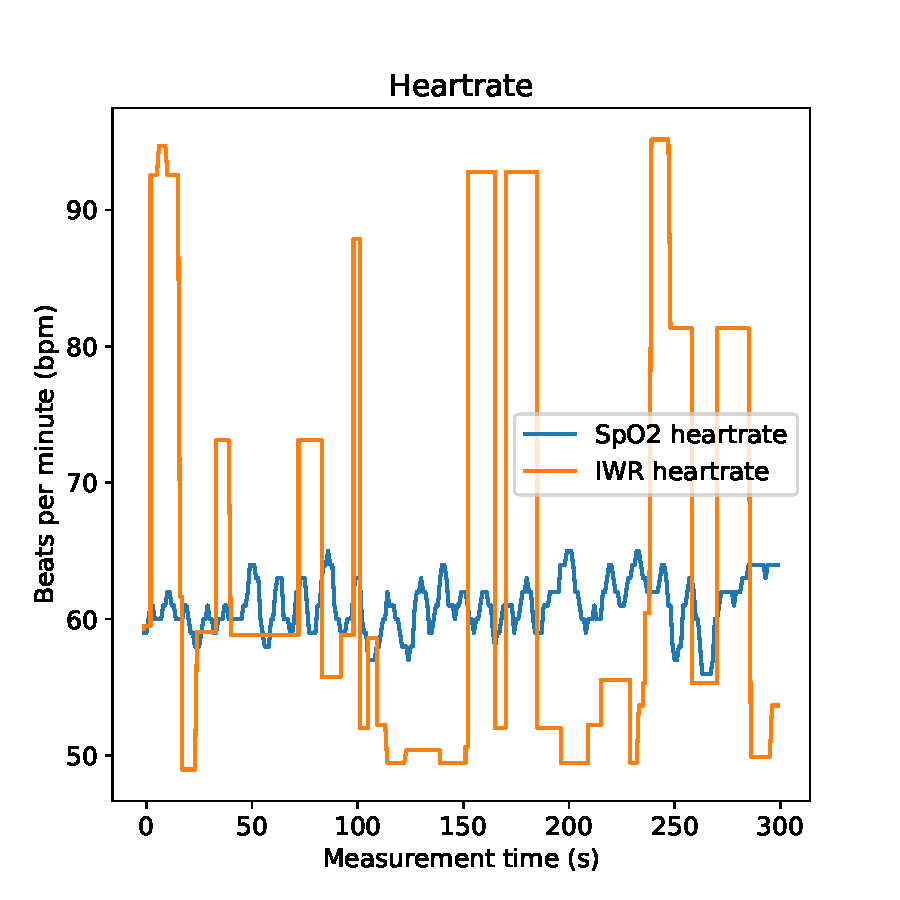
\includegraphics[width=\linewidth]{figures/validation/nick4_heart.pdf}  
  \caption{Heartrate of \emph{P10}}
  \label{fig:nick4_heart}
\end{subfigure}
\begin{subfigure}{.45\textwidth}
  \centering
  % include third image
  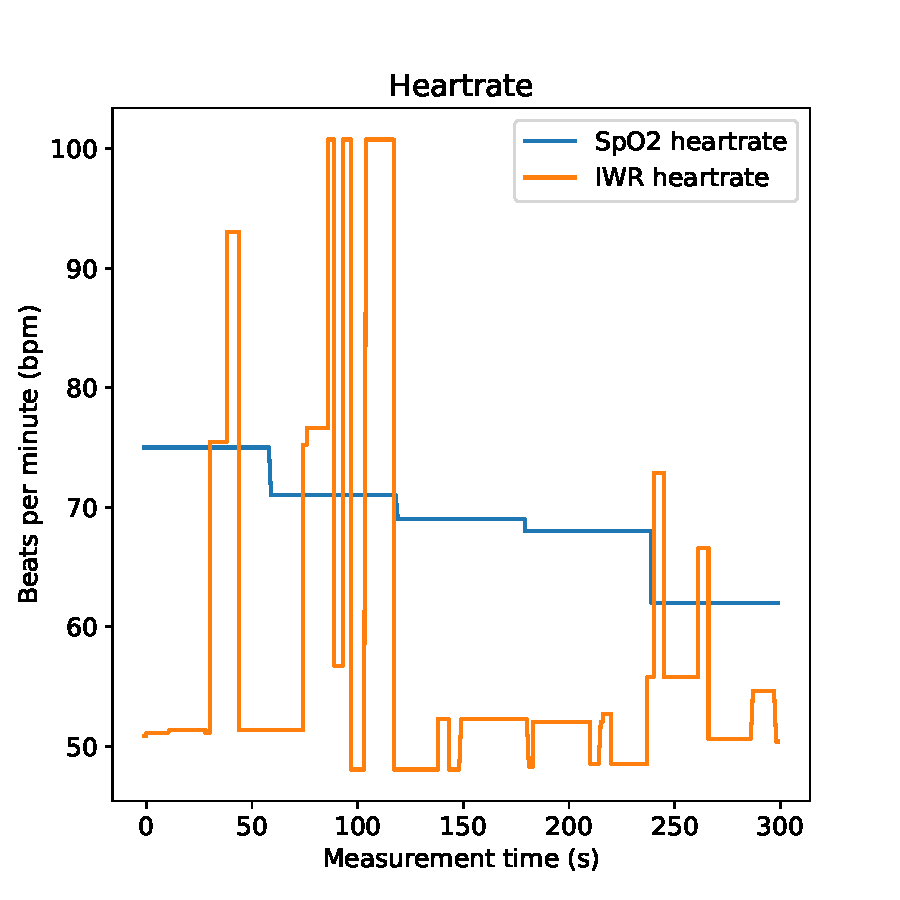
\includegraphics[width=\linewidth]{figures/validation/pascal4_heart.pdf}  
  \caption{Heartrate of \emph{P11}}
  \label{fig:pascal4_heart}
\end{subfigure}
\begin{subfigure}{.45\textwidth}
  \centering
  % include fourth image
  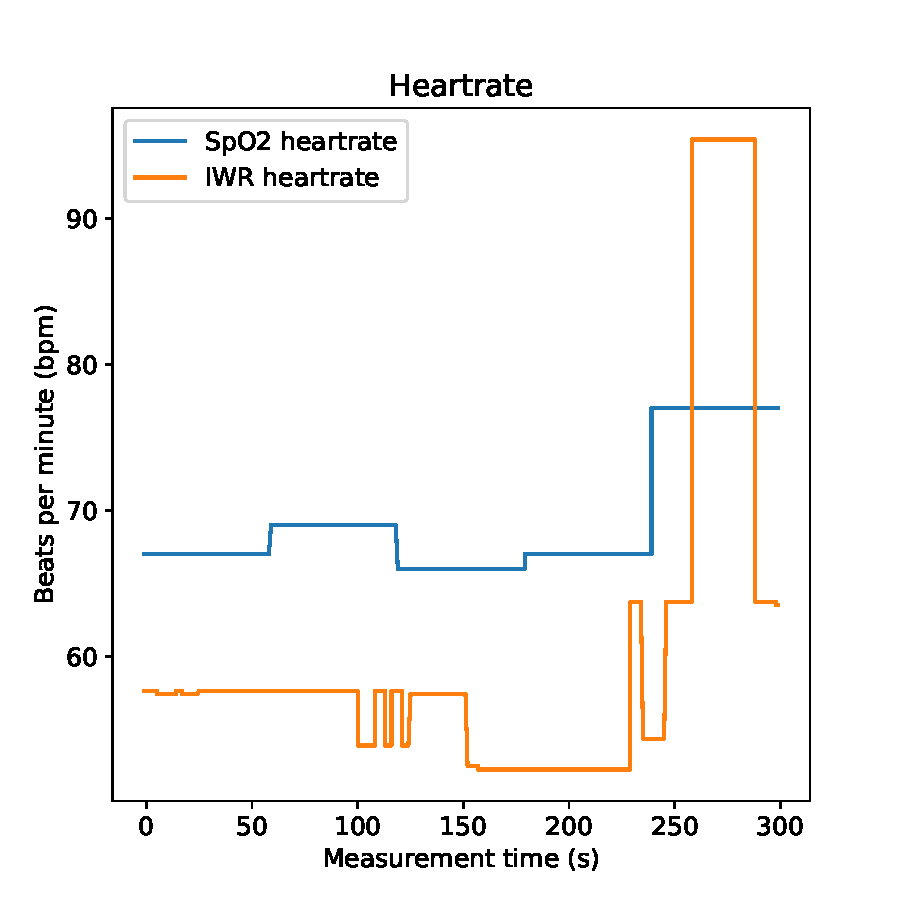
\includegraphics[width=\linewidth]{figures/validation/romy4_heart.pdf}  
  \caption{Heartrate of \emph{P12}}
  \label{fig:romy4_heart}
\end{subfigure}
\caption{Heartrate estimation from 4 persons at the same time.}
\label{fig:4pers_heart_meas}
\end{figure}

\begin{figure}[t]
\centering
\begin{subfigure}{.45\textwidth}
  \centering
  % include first image
  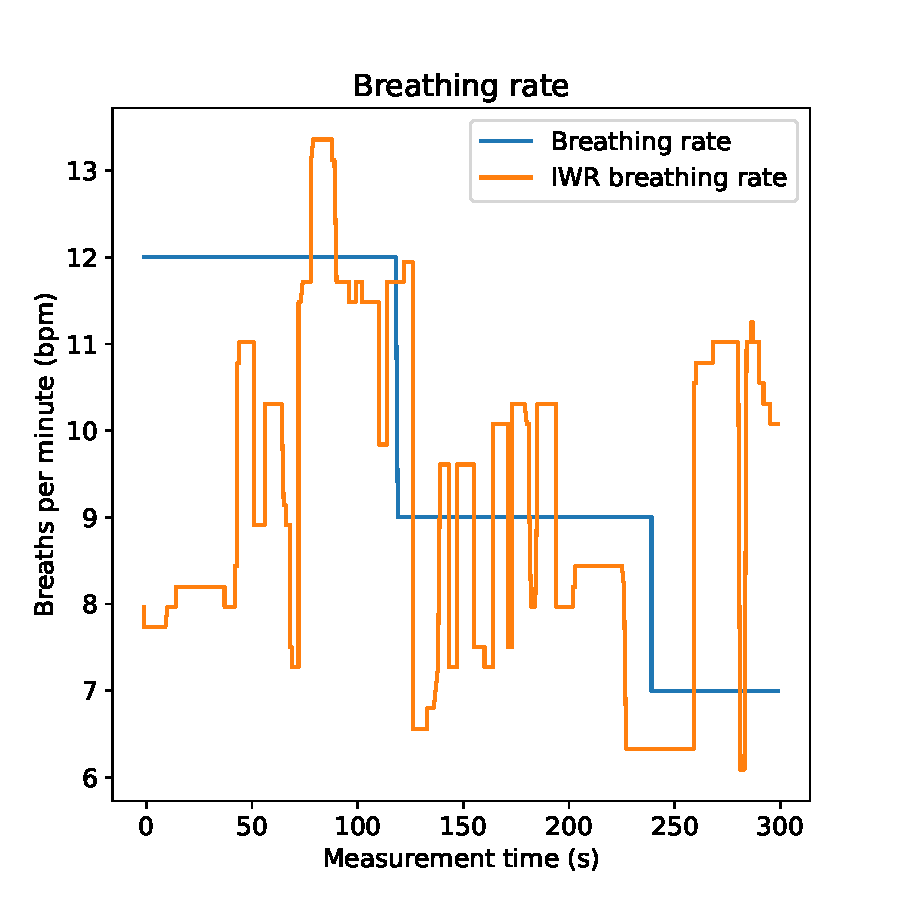
\includegraphics[width=\linewidth]{figures/validation/roy4_breath.pdf}  
  \caption{Respiratory rate of \emph{P3}}
  \label{fig:roy4_breath}
\end{subfigure}
\begin{subfigure}{.45\textwidth}
  \centering
  % include second image
  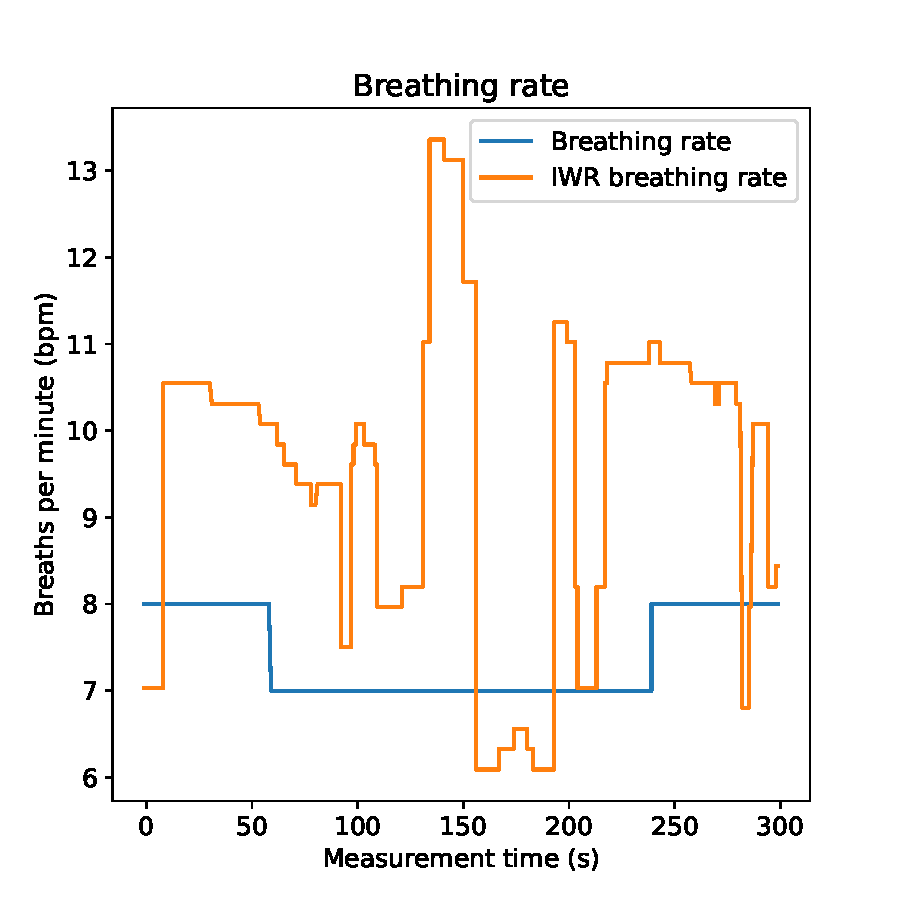
\includegraphics[width=\linewidth]{figures/validation/nick4_breath.pdf}  
  \caption{Respiratory rate of \emph{P10}}
  \label{fig:nick4_breath}
\end{subfigure}
\begin{subfigure}{.45\textwidth}
  \centering
  % include third image
  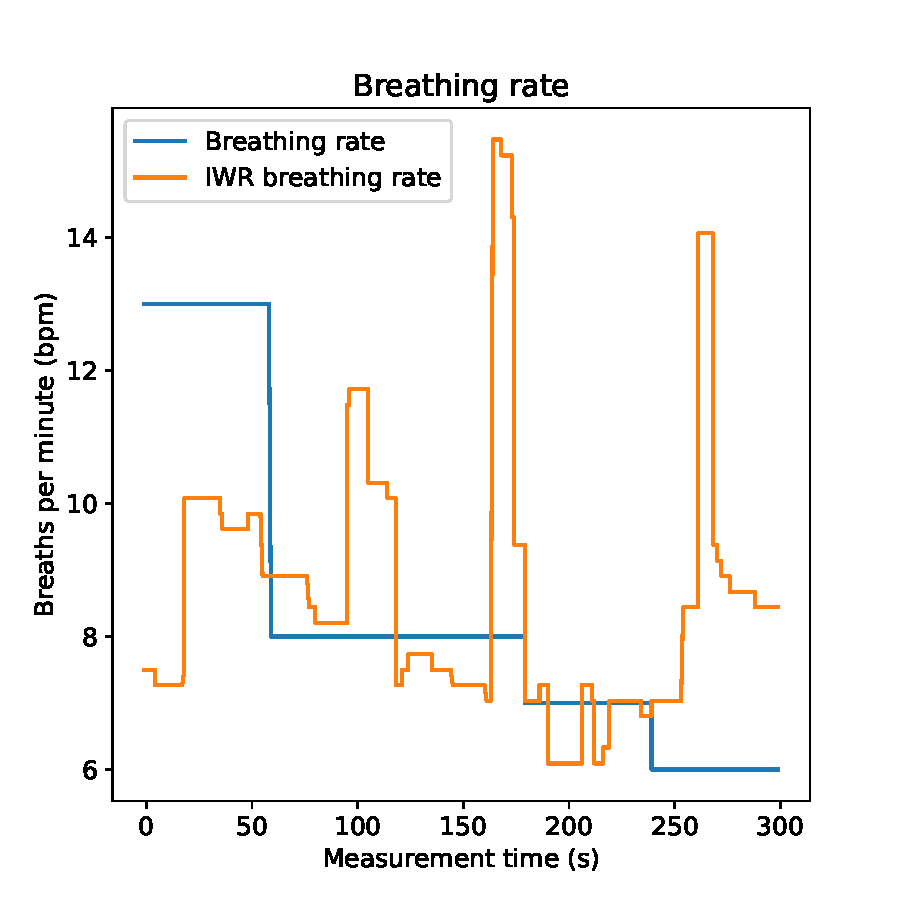
\includegraphics[width=\linewidth]{figures/validation/pascal4_breath.pdf}  
  \caption{Respiratory rate of \emph{P11}}
  \label{fig:pascal4_breath}
\end{subfigure}
\begin{subfigure}{.45\textwidth}
  \centering
  % include fourth image
  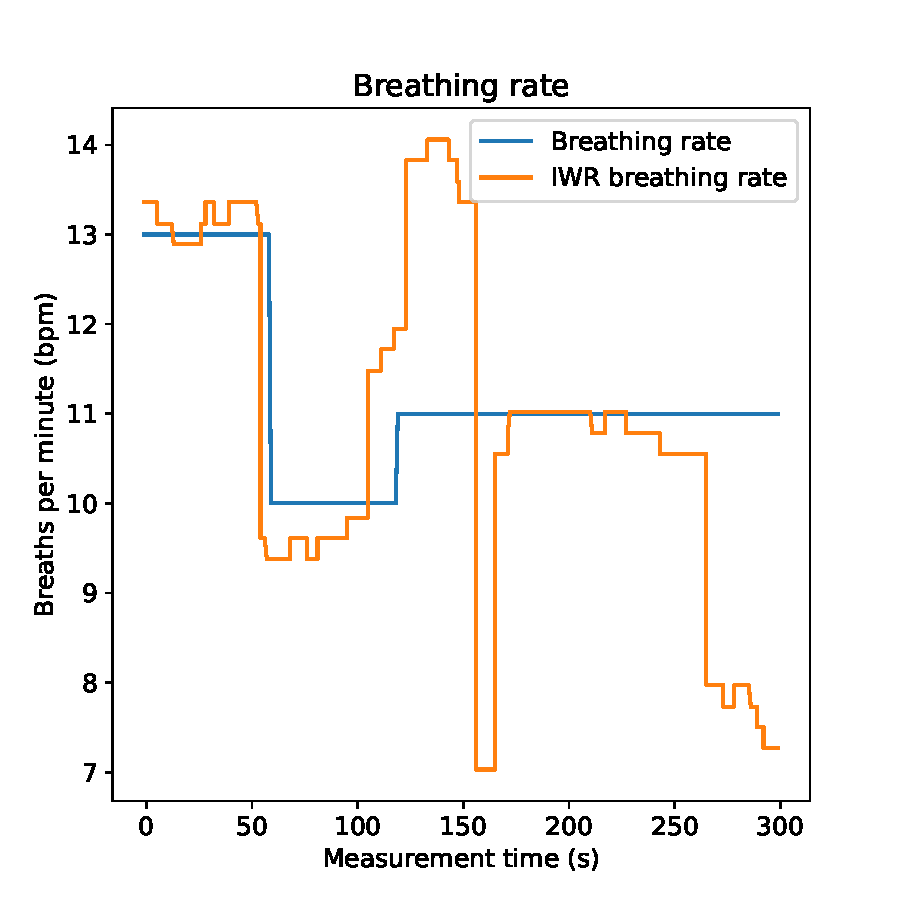
\includegraphics[width=\linewidth]{figures/validation/romy4_breath.pdf}  
  \caption{Respiratory rate of \emph{P12}}
  \label{fig:romy4_breath}
\end{subfigure}
\caption{Respiratory rate estimation from 4 persons at the same time.}
\label{fig:4pers_breath_meas}
\end{figure}

\subsection{Age}

\subsection{Weight}

\subsection{Gender}

\section{Evaluation}
